\documentclass[tikz,border=2mm]{standalone}
\usetikzlibrary{arrows.meta, positioning}

\begin{document}

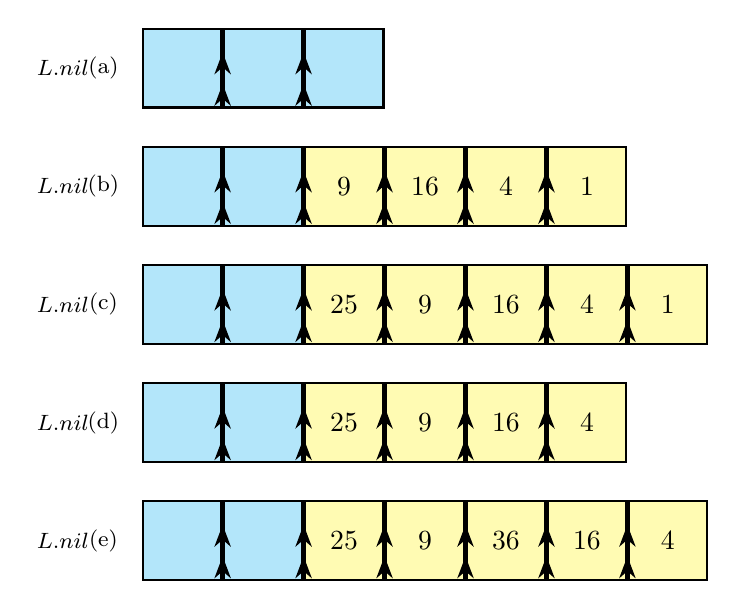
\begin{tikzpicture}[
    box/.style={draw, thick, minimum width=1cm, minimum height=1cm, align=center},
    arrow/.style={-{Stealth[scale=1.2]}, thick},
    textstyle/.style={font=\footnotesize}
]

% Row (a)
\node[textstyle] at (-1, 0) {(a)};
\node[box, fill=cyan!30] (a1) at (0, 0) {};
\node[box, fill=cyan!30, right=0 of a1] (a2) {};
\node[box, fill=cyan!30, right=0 of a2] (a3) {};
\draw[arrow] ([yshift=2mm]a1.east) -- ([yshift=2mm]a2.west);
\draw[arrow] ([yshift=-2mm]a2.west) -- ([yshift=-2mm]a1.east);
\draw[arrow] ([yshift=2mm]a2.east) -- ([yshift=2mm]a3.west);
\draw[arrow] ([yshift=-2mm]a3.west) -- ([yshift=-2mm]a2.east);
\node[textstyle] at ([xshift=-1cm]a1.west) {$L.nil$};

% Row (b)
\node[textstyle] at (-1, -1.5) {(b)};
\node[box, fill=cyan!30] (b1) at (0, -1.5) {};
\node[box, fill=cyan!30, right=0 of b1] (b2) {};
\node[box, fill=yellow!30, right=0 of b2] (b3) {9};
\node[box, fill=yellow!30, right=0 of b3] (b4) {16};
\node[box, fill=yellow!30, right=0 of b4] (b5) {4};
\node[box, fill=yellow!30, right=0 of b5] (b6) {1};
\draw[arrow] ([yshift=2mm]b1.east) -- ([yshift=2mm]b2.west);
\draw[arrow] ([yshift=-2mm]b2.west) -- ([yshift=-2mm]b1.east);
\draw[arrow] ([yshift=2mm]b2.east) -- ([yshift=2mm]b3.west);
\draw[arrow] ([yshift=-2mm]b3.west) -- ([yshift=-2mm]b2.east);
\draw[arrow] ([yshift=2mm]b3.east) -- ([yshift=2mm]b4.west);
\draw[arrow] ([yshift=-2mm]b4.west) -- ([yshift=-2mm]b3.east);
\draw[arrow] ([yshift=2mm]b4.east) -- ([yshift=2mm]b5.west);
\draw[arrow] ([yshift=-2mm]b5.west) -- ([yshift=-2mm]b4.east);
\draw[arrow] ([yshift=2mm]b5.east) -- ([yshift=2mm]b6.west);
\draw[arrow] ([yshift=-2mm]b6.west) -- ([yshift=-2mm]b5.east);
\node[textstyle] at ([xshift=-1cm]b1.west) {$L.nil$};

% Row (c)
\node[textstyle] at (-1, -3) {(c)};
\node[box, fill=cyan!30] (c1) at (0, -3) {};
\node[box, fill=cyan!30, right=0 of c1] (c2) {};
\node[box, fill=yellow!30, right=0 of c2] (c3) {25};
\node[box, fill=yellow!30, right=0 of c3] (c4) {9};
\node[box, fill=yellow!30, right=0 of c4] (c5) {16};
\node[box, fill=yellow!30, right=0 of c5] (c6) {4};
\node[box, fill=yellow!30, right=0 of c6] (c7) {1};
\draw[arrow] ([yshift=2mm]c1.east) -- ([yshift=2mm]c2.west);
\draw[arrow] ([yshift=-2mm]c2.west) -- ([yshift=-2mm]c1.east);
\draw[arrow] ([yshift=2mm]c2.east) -- ([yshift=2mm]c3.west);
\draw[arrow] ([yshift=-2mm]c3.west) -- ([yshift=-2mm]c2.east);
\draw[arrow] ([yshift=2mm]c3.east) -- ([yshift=2mm]c4.west);
\draw[arrow] ([yshift=-2mm]c4.west) -- ([yshift=-2mm]c3.east);
\draw[arrow] ([yshift=2mm]c4.east) -- ([yshift=2mm]c5.west);
\draw[arrow] ([yshift=-2mm]c5.west) -- ([yshift=-2mm]c4.east);
\draw[arrow] ([yshift=2mm]c5.east) -- ([yshift=2mm]c6.west);
\draw[arrow] ([yshift=-2mm]c6.west) -- ([yshift=-2mm]c5.east);
\draw[arrow] ([yshift=2mm]c6.east) -- ([yshift=2mm]c7.west);
\draw[arrow] ([yshift=-2mm]c7.west) -- ([yshift=-2mm]c6.east);
\node[textstyle] at ([xshift=-1cm]c1.west) {$L.nil$};

% Row (d)
\node[textstyle] at (-1, -4.5) {(d)};
\node[box, fill=cyan!30] (d1) at (0, -4.5) {};
\node[box, fill=cyan!30, right=0 of d1] (d2) {};
\node[box, fill=yellow!30, right=0 of d2] (d3) {25};
\node[box, fill=yellow!30, right=0 of d3] (d4) {9};
\node[box, fill=yellow!30, right=0 of d4] (d5) {16};
\node[box, fill=yellow!30, right=0 of d5] (d6) {4};
\draw[arrow] ([yshift=2mm]d1.east) -- ([yshift=2mm]d2.west);
\draw[arrow] ([yshift=-2mm]d2.west) -- ([yshift=-2mm]d1.east);
\draw[arrow] ([yshift=2mm]d2.east) -- ([yshift=2mm]d3.west);
\draw[arrow] ([yshift=-2mm]d3.west) -- ([yshift=-2mm]d2.east);
\draw[arrow] ([yshift=2mm]d3.east) -- ([yshift=2mm]d4.west);
\draw[arrow] ([yshift=-2mm]d4.west) -- ([yshift=-2mm]d3.east);
\draw[arrow] ([yshift=2mm]d4.east) -- ([yshift=2mm]d5.west);
\draw[arrow] ([yshift=-2mm]d5.west) -- ([yshift=-2mm]d4.east);
\draw[arrow] ([yshift=2mm]d5.east) -- ([yshift=2mm]d6.west);
\draw[arrow] ([yshift=-2mm]d6.west) -- ([yshift=-2mm]d5.east);
\node[textstyle] at ([xshift=-1cm]d1.west) {$L.nil$};

% Row (e)
\node[textstyle] at (-1, -6) {(e)};
\node[box, fill=cyan!30] (e1) at (0, -6) {};
\node[box, fill=cyan!30, right=0 of e1] (e2) {};
\node[box, fill=yellow!30, right=0 of e2] (e3) {25};
\node[box, fill=yellow!30, right=0 of e3] (e4) {9};
\node[box, fill=yellow!30, right=0 of e4] (e5) {36};
\node[box, fill=yellow!30, right=0 of e5] (e6) {16};
\node[box, fill=yellow!30, right=0 of e6] (e7) {4};
\draw[arrow] ([yshift=2mm]e1.east) -- ([yshift=2mm]e2.west);
\draw[arrow] ([yshift=-2mm]e2.west) -- ([yshift=-2mm]e1.east);
\draw[arrow] ([yshift=2mm]e2.east) -- ([yshift=2mm]e3.west);
\draw[arrow] ([yshift=-2mm]e3.west) -- ([yshift=-2mm]e2.east);
\draw[arrow] ([yshift=2mm]e3.east) -- ([yshift=2mm]e4.west);
\draw[arrow] ([yshift=-2mm]e4.west) -- ([yshift=-2mm]e3.east);
\draw[arrow] ([yshift=2mm]e4.east) -- ([yshift=2mm]e5.west);
\draw[arrow] ([yshift=-2mm]e5.west) -- ([yshift=-2mm]e4.east);
\draw[arrow] ([yshift=2mm]e5.east) -- ([yshift=2mm]e6.west);
\draw[arrow] ([yshift=-2mm]e6.west) -- ([yshift=-2mm]e5.east);
\draw[arrow] ([yshift=2mm]e6.east) -- ([yshift=2mm]e7.west);
\draw[arrow] ([yshift=-2mm]e7.west) -- ([yshift=-2mm]e6.east);
\node[textstyle] at ([xshift=-1cm]e1.west) {$L.nil$};

\end{tikzpicture}

\end{document}
